\section{Zusammenfassung und Diskussion}

In Versuch 233 beschäftigten wir uns mit der mathematischen Formulierung der Fraunhoferschen Beugung von Licht mit den Werkzeugen der Fourieranalyse. Hierzu betrachteten wir die Beugungs- und Objektbilder eines Einzel- und eines Doppelspalts und verglichen die Lage und Intensitäten der Maxima und Minima der beobachteten Bilder mit den theoretisch vorhergesagten Werten. In der Fourieroptik entspricht das Beugungsbild, welches durch einen Spalt beziehungsweise eine Öffnung, beschrieben durch eine bestimmte Öffnungsfunktion $A$, erzeugt wird, gerade deren Fouriertransformierten 
\begin{gather*}
  E(k_y, k_z) = \int\int_S A(y,z) \e{-i(k_y y + k_z z)} \dy \dz,
\intertext{beziehungsweise im eindimensionalen Fall}
  F(k_y) = \int_{-\infty}^{\infty} f(y) \e{-ik_y y} \dy.\\
\end{gather*}
Umgekehrt lässt sich durch die Rücktransformation vom Beugungsbild auf das Objektbild schließen. Somit ergibt sich als Intensitätsverteilung des Beugungsbildes des Einzelspalts mit der Spaltbreite $d$
\begin{align*}
  I = \sinc(\frac{\pi d}{\lambda} \sin(\alpha))^2 d^2.
\end{align*}
Für den Doppelspalt mit Breite $d$ je Spalt und dem Spaltabstand $g$ ergibt sich
\begin{align*}
  I = 4 \cos(\frac{\pi g}{\lambda} \sin(\alpha))^2 d^2 \sinc(\frac{\pi d}{\lambda} \sin(\alpha))^2.
\end{align*}

Die Versuchsapparatur erlaubte es uns, verschiedene Objekte, also Spalte einzusetzen. Wir verwendeten einen Variablen Einzelspalt, dessen Breite und Rotation sich frei verstellen ließ. Für die Analyse des Doppelspalts verwendeten wir einen von drei gegebenen festen Doppelspalten. Neben diesen war im Strahlengang der Apparatur ein variabler Analysierspalt angebracht, mit welchem wir die Beugungs- und Objektbilder seitlich abschneiden konnten, um so beispielsweise Beugungsmaxima auszublenden.

Wir begannen die Durchführung des Versuchs mit verschiedenen qualitativen Betrachtungen am Einzelspalt. Hierbei untersuchten wir ganz grob die Auswirkungen der Geometrie des Spalts, wie dessen Breite und Rotation, sowie den Einfluss verschiedener Breiten des Analysierspalts auf das Beugungsbild.

Unsere quantitativen Messungen begannen wir zunächst damit, die Abszisse des Intensitätsprofils zu Eichen. Durch den Export aus der Kamerasoftware war diese zunächst in Pixeln angegeben. Hierfür trugen wir die Abstände der Beugungsminima von der ersten bis zur fünften Ordnung (in Pixeln) gegen die jeweils zugehörige Spaltbreite des Analysierspalts (in Millimetern) auf. An diese Daten optimierten wir eine lineare Funktion, deren Steigung von
\begin{align*}
  a &= (8.63 \pm 0.18) \cdot 10^{-4} \frac{\si{\milli\meter}}{\mathrm{px}}
\end{align*}
wir fortan als Umrechnungsfaktor verwendeten.

Wir fuhren fort mit den quantitativen Untersuchungen des Beugungsbildes des Einzelspalts. Hierzu zeichneten wir zunächst zwei Intensitätsverteilungen mit unterschiedlich starken Belichtungszeiten auf. Das erste so, dass das Maximum 0. gerade nicht in Sättigung war, das zweite so, dass die Maxima 1. Ordnung gerade nicht in Sättigung und weitere Maxima höherer Ordnung sichtbar waren. So konnten wir, unter Beachtung der Korrektur durch die Änderung der Belichtungszeit, die Lage und Intensitäten der ersten fünf Maxima und Minima ablesen.

Zunächst trugen wir die Abstände der links- und rechtsseitigen Minima gleicher Ordnung gegen ihre Ordnung in einem Diagramm auf und bestimmten mittels eines Fits die Steigung der daraus resultierenden Gerade. Anhand geometrischer Überlegungen leiteten wir die Gleichung $b = \ffrac{f\lambda}{a}$, um mittels der Brennweite $f$ der Sammellinse , der Wellenlänge $\lambda$ des Lichts und der eben ermittelten Steigung $a$ die Spaltbreite $b$ herzuleiten. Hierbei kamen wir auf einen Wert von 
\begin{align}
  b = (0.262 \pm 0.007)\si{\milli\meter}.
\end{align}
Die tatsächliche Spaltbreite haben wir während den Messungen nicht notiert, daher können wir leider die Abweichung dieses Wertes nicht bestimmen.

Weiter ging es mit der Bestimmung der Ordnungen der Maxima. Da die Abstände der links- und rechtsseitigen Maxima dem gleichen linearen Verhältnis, wie die Minima folgen, konnten wir durch Umkehrung der Proportionalität die Ordnungen der Maxima aus deren Abständen bestimmen. Als Vergleichswerte bestimmten wir numerisch die Positionen der Extrema und zugehörigen Ordnungen anhand der standardmäßigen \texttt{sinc}-Funktion. Die berechneten Werte sind noch einmal in \tabref{tab:es_maxima_ord_ber_vergl_zsmf} zusammengefasst.

\begin{table}[H]
  \centering
  \caption{Abstände der linksseitigen (l) und rechtsseitigen (r) Maxima, die berechneten Ordnungen und Vergleich zu den theoretischen Vorhersagen.}
  \vspace*{0.5em}
  \begin{tabular}{c|c|c|c|c}
    Pixel (l) $\to$ Pixel (r) [px] & Abstand [px] & Ber. Ord. & Theo. Ord. & Abweichung\\\hline
    $273 \pm 4 \to 1305 \pm 4$ & $1032 \pm 6$ & $5.48 \pm 0.04$ & $5.48$ & $0$\\
    $371 \pm 4 \to 1210 \pm 4$ & $839 \pm 6$ & $4.46 \pm 0.04$ & $4.48$ & $0.5\sigma$\\
    $464 \pm 4 \to 1118 \pm 4$ & $654 \pm 6$ & $3.48 \pm 0.04$ & $3.47$ & $0.25\sigma$\\
    $559 \pm 4 \to 1021 \pm 4$ & $462 \pm 6$ & $2.46 \pm 0.04$ & $2.46$ & $0$\\
    $660 \pm 4 \to 924 \pm 4$ & $264 \pm 6$ & $1.40 \pm 0.04$ & $1.43$ & $0.75\sigma$
  \end{tabular}
  \label{tab:es_maxima_ord_ber_vergl_zsmf}
\end{table}

Es ist zu sehen, dass die Ordnungen immer ziemlich genau zwischen den Ordnungen der Minima liegen, so wie es zu erwarten ist und auch von den theoretischen Werten bestätigt wird. Die Abweichungen zur Theorie sind mit unter $1\sigma$ als nicht signifikant zu betrachten.

Im abschließenden Teil zur Betrachtung des Einfachspalts hätten noch die Intensitäten der Maxima 1. bis 5. Ordnung mit den theoretischen Vorhersagen vergleichen müssen. Wie bereits in der Ausarbeitung dieser Aufgabe erklärt hatten wir keine korrekten Daten, um eine Normierung des Intensitätsprofils für den Vergleich durchführen zu können. Eine dieser sehr ähnliche Analyse findet sich allerdings Vollständig im folgenden Versuchsteil zum Doppelspalt wieder.

Einleitend zur Untersuchung des Beugungsbildes des Doppelspalts führten wir erneut zunächst eine qualitative Beobachtung der Auswirkungen verschiedener Geometrien auf das Beugungsbild durch. Hierfür hatten wir einen schmaleren, mittelgroßen und breiten Doppelspalt zur Verfügung. Der schmale Doppelspalt erzeugte ein sehr breites Hauptmaximum mit wenigen Nebenmaxima und kaum sichtbaren weiteren Maxima. Der mittelgroße Doppelspalt zeigte ein etwas schmaleres Hauptmaximum mit etwa drei Nebenmaxima und schwach ausgeprägten weiteren Maxima. Die weiteren quantitativen Untersuchungen führten wir mit dem mittelgroßen Doppelspalt durch.

Das aufgezeichnete Intensitätsprofil des Beugungsbildes, siehe \abbref{fig:ds_gemessen_beugungsbild_zsmf}, verglichen wir zunächst qualitativ mit dem theoretischen, programmatisch erzeugten Beugungsbild und versuchten, die verschiedenen Funktionsanteile, also Gitterfunktion und Spaltfunktion in diesem zu verorten.

\begin{figure}[H]
  \centering
  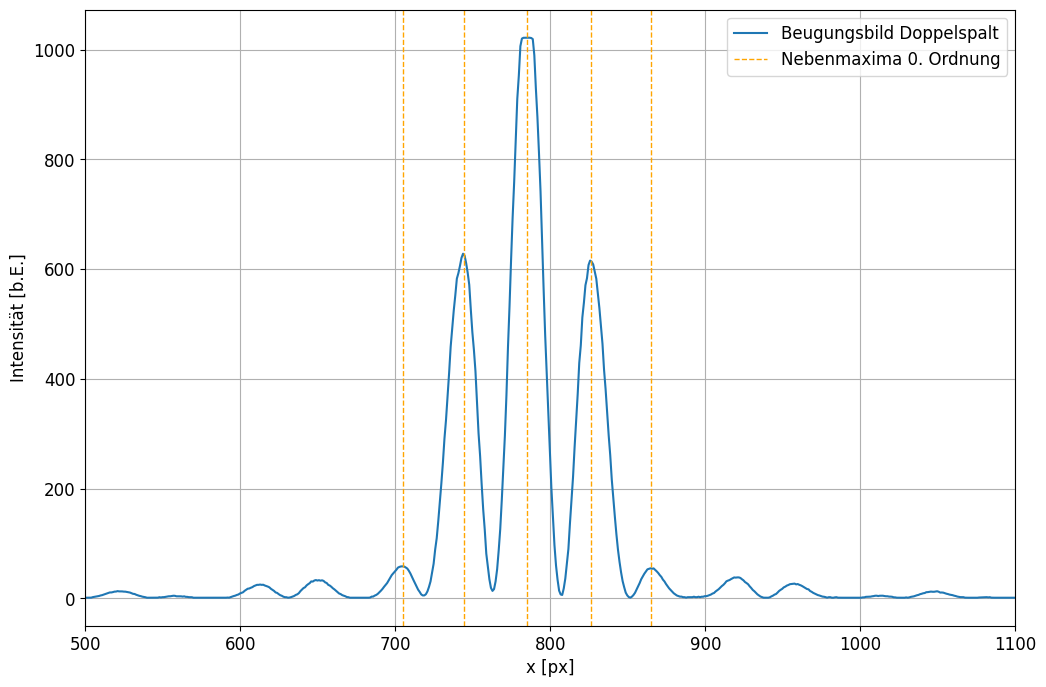
\includegraphics[width=.9\textwidth]{files/plots/3/ds_gemessen_beugungsbild.png}
  \caption{Gemessenes Beugungsbild des Doppelspalts.}
  \label{fig:ds_gemessen_beugungsbild_zsmf}
\end{figure}

Im zweiten Teil betrachteten wir die Intensität der Nebenmaxima des 0. Hauptmaximums, in \abbref{fig:ds_gemessen_beugungsbild_zsmf} markiert, genauer. Wie bereits beim Einzelspalt (\textit{hätten wir gescheit gemessen}) , entnahmen wir aus den Daten die Intensitäten der Nebenmaxima und normierten diese auf die Intensität des 0. Hauptmaximum. Erneut numerisch, ermittelten wir dann die theoretisch erwarteten Werte der Intensitäten, ebenfalls auf das Hauptmaximum normiert und verglichen diese mit unseren Messwerten. Die Resultate sind nochmals in \tabref{tab:es_vergleich_intensitaet_zsmf} zusammengefasst.

\begin{table}[H]
  \centering
  \caption{Vergleich der Intensitäten der Nebenmaxima des 0. Hauptmaximums beim Einzelspalt.}
  \vspace*{0.5em}
  \begin{tabular}{|c|c|c|c|c|}\hline
    Ordnung & Intensität & Intensität (normiert) & Intensität (theo.) & Abw.\\\hline
    \multicolumn{5}{|l|}{Linksseitige Maxima}\\\hline
    1 & $628 \pm 2$   & $0.6146 \pm 0.0021$    &  $0.5417 \pm 0.0001$     &   $35.52\sigma$\\
    2 & $58 \pm 2$    & $0.0568 \pm 0.0020$    &  $0.0448 \pm 0.0001$     &   $6.1\sigma$\\\hline
    \multicolumn{5}{|l|}{Rechtsseitige Maxima}\\\hline
    1 & $616 \pm 2$  &  $0.6028 \pm 0.0021$    &  $0.5417 \pm 0.0001$   &     $29.84\sigma$\\
    2 & $55 \pm 2$   &  $0.0538 \pm 0.0020$    &  $0.0448 \pm 0.0001$   &     $4.61\sigma$\\\hline
  \end{tabular}
  \label{tab:es_vergleich_intensitaet_zsmf}
\end{table}

Während die Abweichungen der Intensitäten der Maxima 2. Ordnung noch in einem groben Rahmen halten, verzeichnen wir bei den Maxima erster Ordnung Abweichungen um $30\sigma$ von der Theorie.